\documentclass[10pt,a4paper]{report}
\usepackage[utf8]{inputenc}
\usepackage[russian]{babel}
\usepackage{amsmath}
\usepackage{amsfonts}
\usepackage{amssymb}
\usepackage{graphicx}
\usepackage{hyperref}
\renewcommand{\thesection}{\arabic{section}}
\setcounter{totalnumber}{10}
\setcounter{topnumber}{10}
\setcounter{bottomnumber}{10}
\renewcommand{\topfraction}{1}
\renewcommand{\textfraction}{0}
\author{Климов Сергей}
\title{Лабораторная работа №3.\\
	Программа для шифрования и подписи GPG, пакет Gpg4win}
\begin{document}
\maketitle
\tableofcontents
\pagebreak

\section{Цель работы}
Научиться создавать сертификаты, шифровать файлы и ставить ЭЦП.
\section{Описание работы}
Цифровой сертификат – это электронный документ, который выдается и заверяется Центром Сертификации (ЦС). Для заверения электронного сертификата используется электронная цифровая подпись доверенного центра, т.е. Центра Сертификации.  Цифровой сертификат выдается физическому лицу, который является владельцем закрытого ключа электронной цифровой записи (шифрования), который соответствует открытому ключу.
Цифровой сертификат содержит следующую информацию: имя и идентификатор владельца сертификата, открытый ключ подписи, имя, идентификатор и цифровую подпись Центра Сертификации, серийный номер, версию и срок действия сертификата.
Владелец сертификата может быть уверен, что информация, которая передается им электронным способом, не будет прочитана, похищена или подменена во время ее передачи через интернет.
\href {goo.gl/W4FzmI}{securitylab.ru}

Шифрование – метод, используемый для преобразования данных в шифрованный текст для того, чтобы они были прочитаны только пользователем, обладающим соответствующим ключом шифрования для расшифровки содержимого. Шифрование используется тогда, когда требуется повышенный уровень защиты данных - при хранении данных в ненадежных источниках или передачи данных по незащищенным каналам связи.
В зависимости от структуры используемых ключей, среди методов шифрования выделяют симметричное шифрование и асимметричное шифрование. Симметричное шифрование предусматривает доступность алгоритма шифрования посторонним лицам, однако ключ (одинаковый для отправителя и получателя) остается неизвестным. При ассиметричном шифровании посторонним лицам известен алгоритм шифрования и открытый ключ, однако закрытый ключ известный только получателю.
\href {goo.gl/BBLQN1}{securitylab.ru}

Электронная цифровая подпись (ЭЦП) - это реквизит электронного документа, предназначенный для защиты данного электронного документа от подделки, полученный в результате криптографического преобразования информации с использованием закрытого ключа электронной цифровой подписи и позволяющий идентифицировать владельца сертификата ключа подписи, а также установить отсутствие искажения информации в электронном документе, а также обеспечивает неотказуемость подписавшегося. 
\href {goo.gl/2nEYGZ}{russika.ru}

При выполнении лабораторной работы для создания сертификатов, шифрования и создания ЭЦП используется пакет
Gpg4win. Он включает в себя:
\begin{itemize}
\item версию GnuPG — свободная программа для шифрования информации и создания электронных цифровых подписей;
\item Kleopatra (менеджер сертификатов для OpenPGP и X.509);
\item GPA (альтернативный менеджер сертификатов (GNU) для OpenPGP и X.509);
\item другие компоненты.
\end{itemize}
\pagebreak
\section{Ход работы}
Для работы будем использовать графическую оболочку \textbf{"Kleopatra"}.
\subsection{Создание ключевой пары openPGP}
Для создания новой ключевой пары OpenPGP была выполнена команда \textit{"File -> New Certificate"}. После чего была введена персональная информация: имя сертификата, адрес электронной почты пользователя.% (рисунок %\ref{ris:image1} ).
%\begin{figure}[ht]	\center{\includegraphics[width=0.8\linewidth]{image/1}}
%\caption{Окно для ввода персональных данных.}\label{ris:image1}
%\end{figure}

%Далее подтвердим персональные данные, нажав кнопку \textit{"Create Key"} (рисунок \ref{ris:image2} ).
%\begin{figure}[ht]	\center{\includegraphics[width=0.8\linewidth]{image/2}}
%\caption{Окно создания ключа.}
%\label{ris:image2}
%\end{figure}

%После необходимо дважды ввести фразу-пароль (рисунок \ref{ris:image3} ).

%\begin{figure}[h]
%\parbox[b]{0.3\linewidth}
%{\centering
%    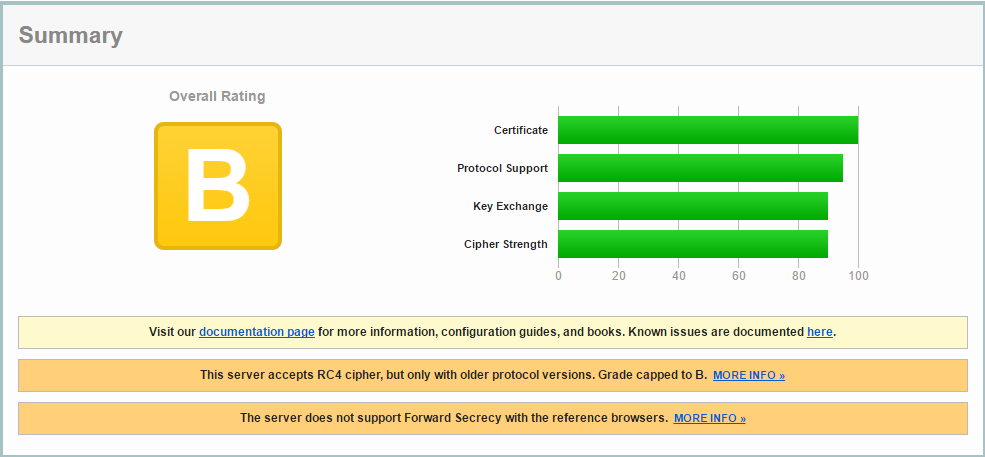
\includegraphics{image/3}}
%\hspace*{\fill}
%\parbox[b]{0.3\linewidth}
%{\centering
%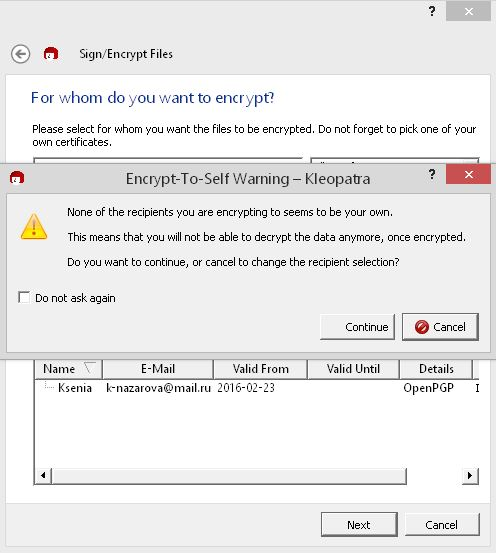
\includegraphics{image/4}}
% \caption{Окно ввода и подтверждения фразы-пароля}
%\label{ris:image3}
%\end{figure}

%Сертификат успешно создан (рисунок  \ref{ris:image4} ).
%\begin{figure}[h]
%\center{\includegraphics[width=1\linewidth]{image/5}}
%\caption{Созданный сертификат}
%\label{ris:image4}
%end{figure}

После этого созданный сертификат был импортирован в рафическую оболочку \textbf{"Kleopatra"} (рисунок  \ref{ris:image1} ).

\begin{figure}[ht]	\center{\includegraphics[width=0.8\linewidth]{images/1}}
\caption{Окно для ввода персональных данных.}\label{ris:image1}
\end{figure}

\subsection{Экспорт сертификата}
Для экспорта сертификата выполним команду \textit{"File ->  Export Certificate"}.

\subsection{Поставить ЭЦП на файл}
Для того, что бы поставить ЭЦП на файл была выполнена команда \textit{"File -> Sign/Encrypt Files"}, затем был выбран файл, на который необходимо поставить ЭЦП.

После выберем одно из трех предложенных действий.
\begin{itemize}
\item Sign and Encrypt
\item Encrypt
\item Sign
\end{itemize} 

Был выбран пункт \textit{Sign and Encrypt} - создание цифровой подписи и шифрование файла (рисунок \ref{ris:image2} ).\\
\begin{figure}[h]
\center{\includegraphics[width=0.6\linewidth]{images/2}}
\caption{Поставить ЭЦП на файл и зашфровать}
\label{ris:image2}
\end{figure}

Был выбран открытый ключ получателя (рисунок \ref{ris:image3} ).\\

\begin{figure}[h]
\center{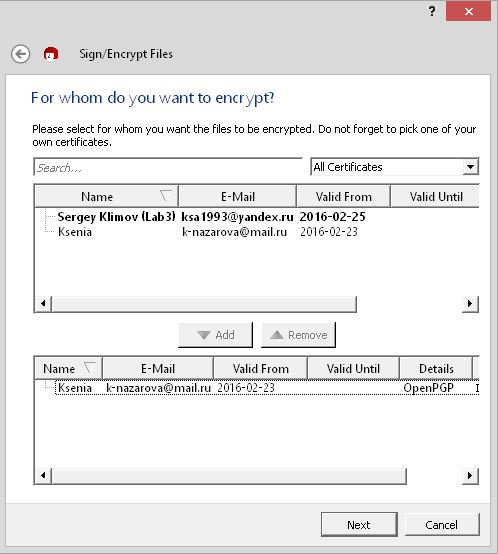
\includegraphics[width=0.6\linewidth]{images/3}}
\caption{Выбор открытого ключа получателя}
\label{ris:image3}
\end{figure}

Был выбран стандарт OpenPGP для подписи и сертификат, созданный ранее (рисунок \ref{ris:image4} ).\\
\begin{figure}[h]	\center{\includegraphics[width=0.8\linewidth]{images/5}}
\caption{Выбор стандарта OpenPGP и сертификата для ЭЦП}
\label{ris:image4}
\end{figure}
\pagebreak
После ввода пароля выводится сообщение об успешном создании подписи на файл (рисунок \ref{ris:image5} ).
\begin{figure}[h]	\center{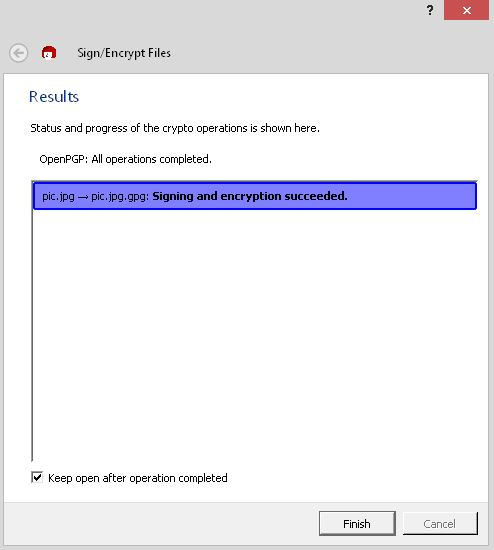
\includegraphics[width=0.8\linewidth]{images/6}}
\caption{Успешная подпись файла}
\label{ris:image5}
\end{figure}
\newpage
%\pagebreak
%\bigskip
\subsection{Работа с чужим сертификатом}
Был импортирован сторонний сертификат, после этого с его помощью был зашифрован и подписан документ \textit{pic.jpg}. Далее зашифрованный файл \textit{pic.jpg.gpg} был отправлен коллеге для расшифровки. \\
Далее от коллеги был получен файл \textit{hello.txt.gpg}, который был подписан при помощи моего открытого ключа. Затем командой \textit{File -> Decrypt/Verify Files} расшифруем документ (рисунок \ref{ris:image6} ). 
\begin{figure}[h]	\center{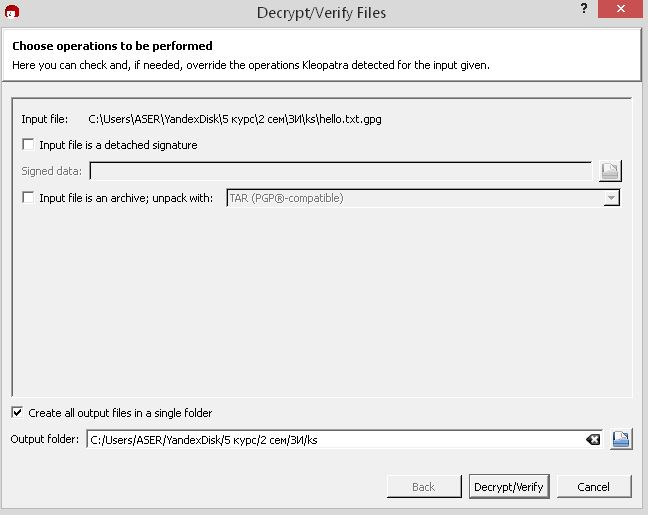
\includegraphics[width=0.7\linewidth]{images/7}}
\caption{Расшифровка файла}
\label{ris:image6}
\end{figure}

После ввода пароля видим окно с сообщением об удачном расшифровании файла 
(рисунок \ref{ris:image7} ), также появился файл \textit{hello.txt}, который можно прочитать.
\begin{figure}[h]	\center{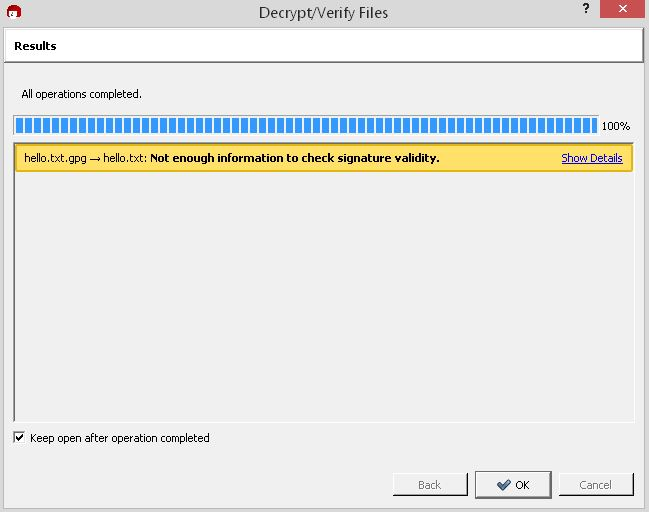
\includegraphics[width=0.7\linewidth]{images/8}}
\caption{Успешное расшифрование файла}
\label{ris:image7}
\end{figure}
\newpage
\subsection{Использование GNU Privacy handbook}
С помощью GNU Privacy handbook проделаем некоторые действия по использованию gpg через командную строку. \\
Для создания ключевой пары введем в консоле команду \textit{gpg --gen-key}. Далее выберем тип ключа, его размер, срок действия, укажем ID пользователя, электронную почту, введем пароль, после чего создастся ключевая пара.\\
Был создан ключ типа RSA, размером 2048, с неограниченным сроком действия (рисунок \ref{ris:image8} ). \\
\pagebreak
\begin{figure}[h]	\center{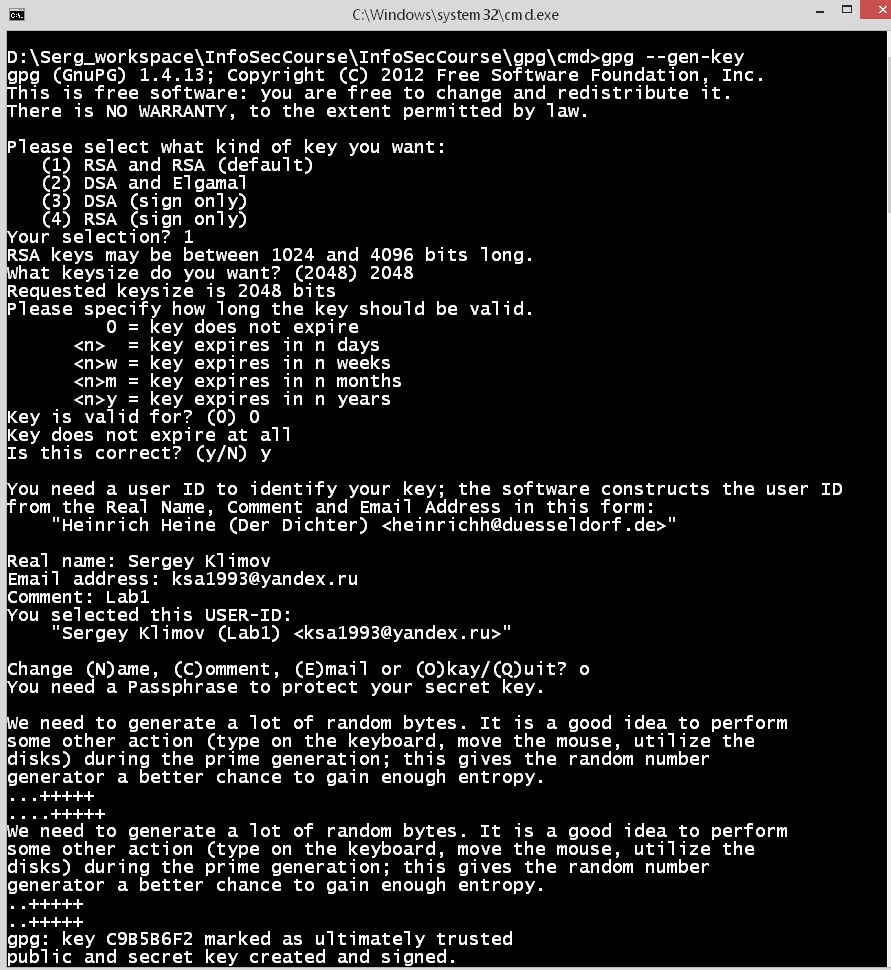
\includegraphics[width=0.8\linewidth]{images/9}}
\caption{Создание сертификата}
\label{ris:image8}
\end{figure}
 
Выведем список всех ключей командой \textit{gpg --list-keys} (рисунок \ref{ris:image9} ). \\
\begin{figure}[h]	\center{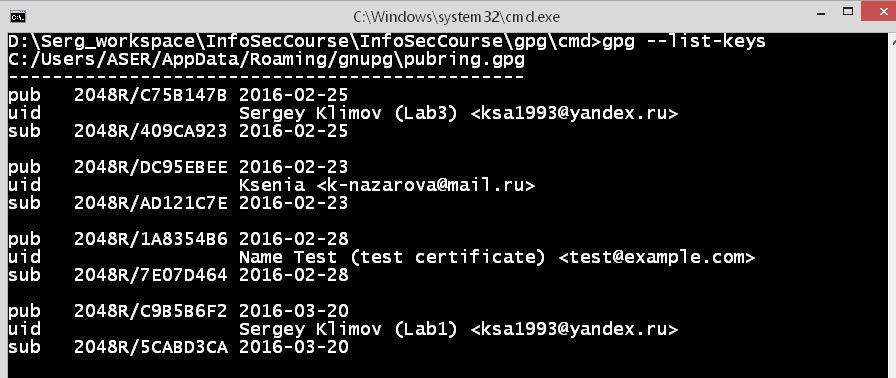
\includegraphics[width=0.8\linewidth]{images/10}}
\caption{Список сертификатов}
\label{ris:image9}
\end{figure}
\pagebreak
Подпишем файл \textit{pic.jpg} (рисунок \ref{ris:image10} ). \\

\begin{figure}[h]	\center{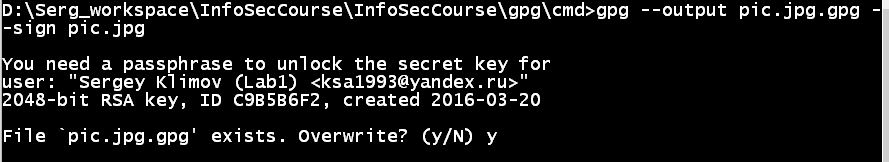
\includegraphics[width=0.8\linewidth]{images/11}}
\caption{Создание сертификата}
\label{ris:image10}
\end{figure}

Выведем на консоль содеожимое файла сертификата (рисунок \ref{ris:image11} ).\\

\begin{figure}[h]	\center{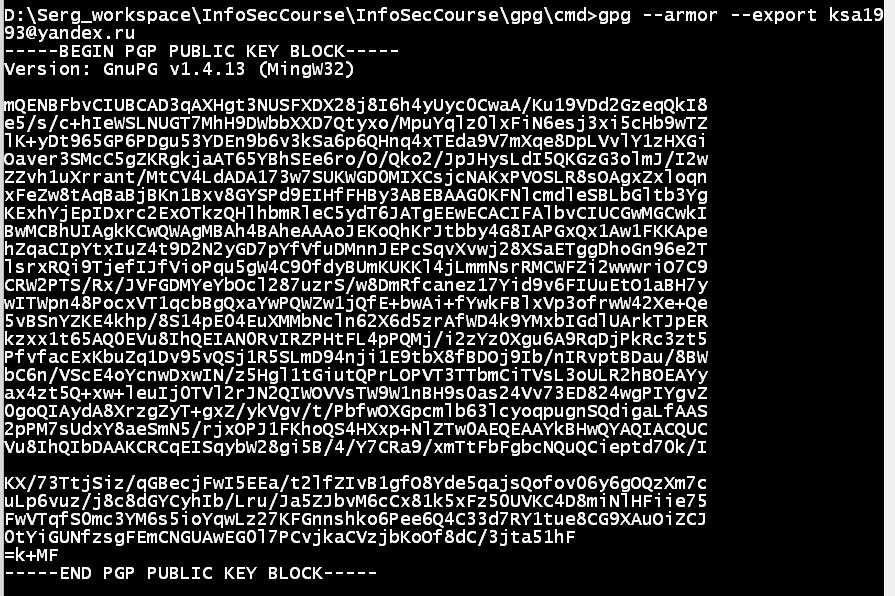
\includegraphics[width=0.8\linewidth]{images/12}}
\caption{Содержимое файла сертификата}
\label{ris:image11}
\end{figure}

\section{Вывод}
В результате выполнения лабораторной работы был изучен пакет Gpg4win. Были получены практические навыки создания ключевых пар,  подписи, шифрования и дешифрования файлов при помощи графической оболчки \textbf{Kleopatra}, а также при помощи консольной утилиты \textbf{gpg}.
\end{document}
